\documentclass[spanish]{beamer}

\include{conf/preconfig}
\include{conf/packages}
\include{conf/config}
\include{beamerconf}
%
%
\usetheme{Bergen}
\usecolortheme{orchid}
%
%
%
\title{Identificación de edificios y monumentos a partir de fotografías tomadas 
con dispositivos móviles}
\author{Esteban C. Fornal \and Christian N. Pfarher \and Mauro J. Torrez}
\date{\today}

\begin{document}
%
\frame{\titlepage}

%%%%%%%%%%%%%%%%%%%%%%%%%%%%%%%%%%%%%%%%%%%%%%%%%%%%%%%%%
\section[Outline]{Objetivo}

\begin{frame}{}
\frametitle{Objetivo}
Identificar edificios y monumentos a partir de fotografías
\end{frame}

%%%%%%%%%%%%%%%%%%%%%%%%%%%%%%%%%%%%%%%%%%%%%%%%%%%%%%%%%
\section[Outline]{Herramientas}

\begin{frame}{Técnicas:}
\begin{itemize}
\item<1-> Transformada de Hough
\item<2-> Histograma
\end{itemize}
\end{frame}

%%%%%%%%%%%%%%%%%%%%%%%%%%%%%%%%%%%%%%%%%%%%%%%%%%%%%%%%%
\section[Outline]{Técnicas}

\begin{frame}{Transformada de Hough}
  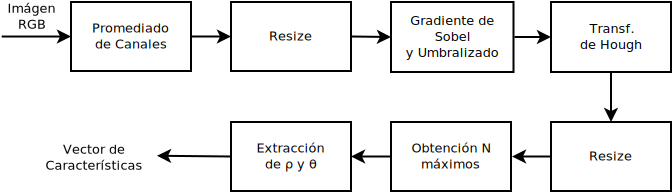
\includegraphics[width=9cm]{../diagramas/procesohough}

  \begin{itemize}
  \item[]
    \begin{equation*}
      \label{umbral}
      f(I)=
      \begin{cases}
      0, & I\leq U\\
      255, & I > U
      \end{cases}
      \end{equation*}
  \item 60 características
  \end{itemize}
\end{frame}

\begin{frame}{Histograma}
  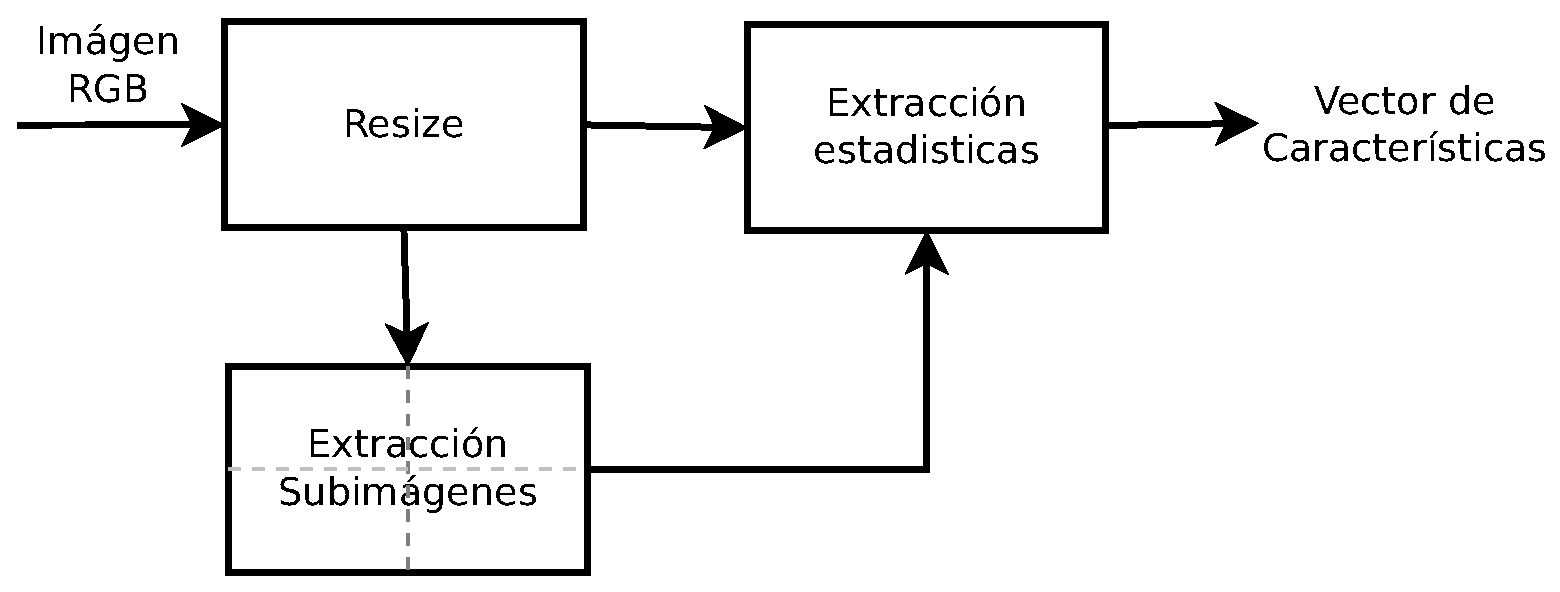
\includegraphics[width=9cm]{../diagramas/procesoestadisticas}
  \begin{itemize}
  \item 45 características
  \end{itemize}
\end{frame}

%%%%%%%%%%%%%%%%%%%%%%%%%%%%%%%%%%%%%%%%%%%%%%%%%%%%%%%%%
\section[Outline]{Métodos}

\begin{frame}{Entrenamiento}
  \begin{itemize}
  \item Etiquetado de imágenes
  \item Generación de prototipos
  \end{itemize}
\end{frame}

\begin{frame}{Clasificación}
  \begin{itemize}
  \item Error cuadrático medio
    \begin{align*}
      MSE = \frac{1}{MN} \sum_x\sum_y [ f(x,y) - g(x,y) ]^{2}
    \end{align*}
  \item Obtención de la Clase
  \end{itemize}
\end{frame}

%%%%%%%%%%%%%%%%%%%%%%%%%%%%%%%%%%%%%%%%%%%%%%%%%%%%%%%%%
\section[Outline]{Pruebas}

\begin{frame}{Armado Base de Datos}
  \begin{itemize}
  \item Imágenes de 640x480
  \item Obtenidas con celular
  \item Diurnas y nocturnas 
  \end{itemize}
\end{frame}

%%%%%%%%%%%%%%%%%%%%%%%%%%%%%%%%%%%%%%%%%%%%%%%%%%%%%%%%%
\section[Outline]{Resultados}

\begin{frame}{Resultados}
  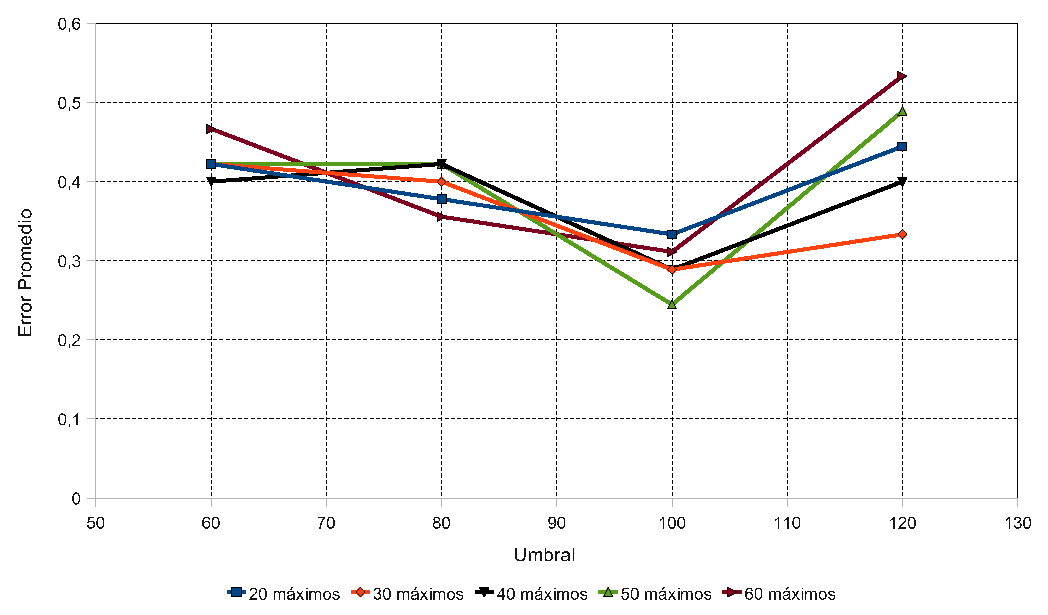
\includegraphics[width=9cm]{../diagramas/estadistica_noche_iguales}
\end{frame}

%%%%%%%%%%%%%%%%%%%%%%%%%%%%%%%%%%%%%%%%%%%%%%%%%%%%%%%%%
\section[Outline]{Conclusiones}

\begin{frame}{Conclusiones}
  \begin{itemize}
  \item Sensores
    \begin{itemize}
    \item Cantidad
    \item Tipo
    \item Configuración
    \end{itemize}
  \item Resultados satisfactorios para la información disponible
  \end{itemize}
\end{frame}

\end{document}








